\pdfminorversion=4
\documentclass[aspectratio=169]{beamer}

\mode<presentation>
{
  \usetheme{default}
  \usecolortheme{default}
  \usefonttheme{default}
  \setbeamertemplate{navigation symbols}{}
  \setbeamertemplate{caption}[numbered]
  \setbeamertemplate{footline}[frame number]  % or "page number"
  \setbeamercolor{frametitle}{fg=white}
  \setbeamercolor{footline}{fg=black}
} 

\usepackage[english]{babel}
\usepackage{inputenc}
\usepackage{tikz}
\usepackage{courier}
\usepackage{array}
\usepackage{bold-extra}
\usepackage{minted}
\usepackage[thicklines]{cancel}
\usepackage{fancyvrb}

\xdefinecolor{dianablue}{rgb}{0.18,0.24,0.31}
\xdefinecolor{darkblue}{rgb}{0.1,0.1,0.7}
\xdefinecolor{darkgreen}{rgb}{0,0.5,0}
\xdefinecolor{darkgrey}{rgb}{0.35,0.35,0.35}
\xdefinecolor{darkorange}{rgb}{0.8,0.5,0}
\xdefinecolor{darkred}{rgb}{0.7,0,0}
\definecolor{darkgreen}{rgb}{0,0.6,0}
\definecolor{mauve}{rgb}{0.58,0,0.82}

\title[2023-05-09-chep23-analysis-of-physicists]{Analysis of physics analysis}
\author{Jim Pivarski}
\institute{Princeton University -- IRIS-HEP}
\date{May 9, 2023}

\usetikzlibrary{shapes.callouts}

\begin{document}

\logo{\pgfputat{\pgfxy(0.11, 7.4)}{\pgfbox[right,base]{\tikz{\filldraw[fill=dianablue, draw=none] (0 cm, 0 cm) rectangle (50 cm, 1 cm);}\mbox{\hspace{-8 cm}\includegraphics[height=1 cm]{princeton-logo-long.png}\hspace{0.1 cm}\raisebox{0.1 cm}{\includegraphics[height=0.8 cm]{iris-hep-logo-long.png}}\hspace{0.1 cm}}}}}

\begin{frame}
  \titlepage
\end{frame}

\logo{\pgfputat{\pgfxy(0.11, 7.4)}{\pgfbox[right,base]{\tikz{\filldraw[fill=dianablue, draw=none] (0 cm, 0 cm) rectangle (50 cm, 1 cm);}\mbox{\hspace{-8 cm}\includegraphics[height=1 cm]{princeton-logo.png}\hspace{0.1 cm}\raisebox{0.1 cm}{\includegraphics[height=0.8 cm]{iris-hep-logo.png}}\hspace{0.1 cm}}}}}

% Uncomment these lines for an automatically generated outline.
%\begin{frame}{Outline}
%  \tableofcontents
%\end{frame}

%% https://indico.jlab.org/event/459/contributions/11547/

%% Analysis of physics analysis
%%  9 May 2023, 16:00
%%  15m
%%  Marriott Ballroom VI-VII (Norfolk Waterside Marriott)

%% Speaker
%%  Pivarski, Jim (Princeton University)
%% Description
%% Data analysis in particle physics is socially distributed: unlike centrally developed and executed reconstruction pipelines, the analysis work performed after Analysis Object Descriptions (AODs) are made and before the final paper review—which includes particle and event selection, systematic error handling, decay chain reconstruction, histogram aggregation, fitting, statistical models, and machine learning—are often performed “off the GRID.”

%% This presents a challenge for developers of analysis tools, who need to know how their tools are being used in order to focus efforts in development, documentation, and training. The most common methods have traditionally been direct conversations with known users, wide-cast surveys, and download counts, but each of these has its limitations.

%% In this talk, I will discuss the above as well as new methods of analyzing user behavior: collecting issue comments through GitHub and GitLab APIs, statically analyzing code from thousands of git repositories matching search criteria, and web analytics of documentation sites. Applying these methods to the Awkward Array library reveals the most commonly used functions, slice idioms, and data types, as well as what libraries Awkward Array is commonly used with and how data are transferred between them. Finally, I apply these methods to other physics analysis libraries to show the generality of the techniques.

%% Consider for long presentation	No

% START START START START START START START START START START START START START

\begin{frame}{Dark computing}
\vspace{0.25 cm}
\begin{columns}
\column{1.1\linewidth}
\only<1>{\includegraphics[width=\linewidth]{PLOTS/analysis-chain-0.pdf}}\only<2->{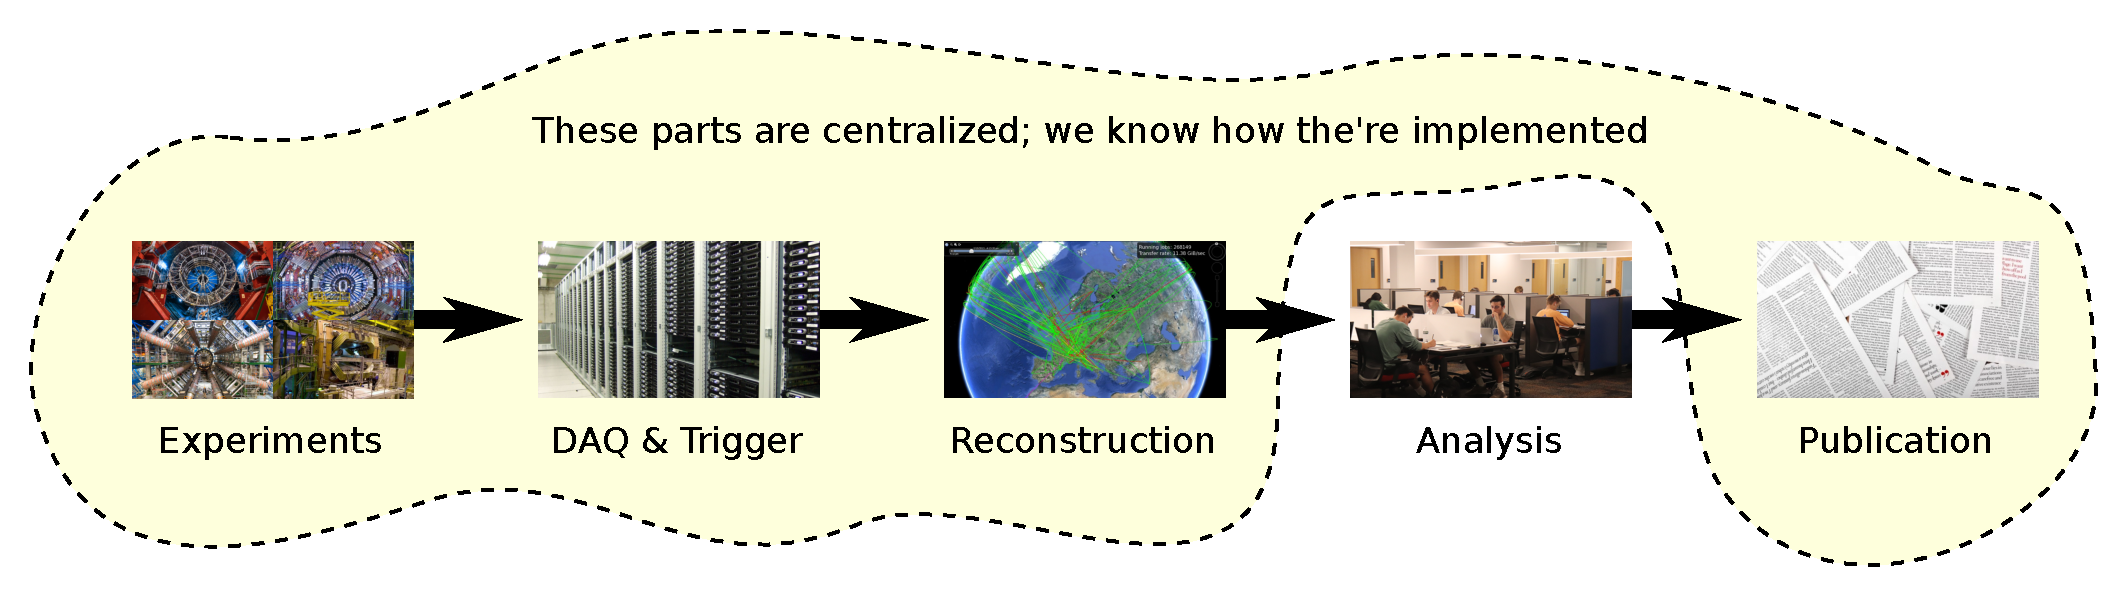
\includegraphics[width=\linewidth]{PLOTS/analysis-chain.pdf}}
\end{columns}

\vspace{0.5 cm}
\begin{itemize}
\item<3-> Good software depends on mutual understanding (between developers and users) of what the software is for and how it's supposed to be used.
\item<4-> The ``analysis'' step is the only one in the pipeline for which we don't even know \underline{\it who} all the users are.
\end{itemize}
\end{frame}

\begin{frame}{We don't do this}
\vspace{1 cm}
\begin{center}
\includegraphics[width=0.5\linewidth]{PLOTS/iphone-send-usage-data.png}
\end{center}
\end{frame}

\begin{frame}{So what can we do instead?}
\vspace{0.35 cm}
\begin{columns}
\column{1.05\linewidth}

\renewcommand{\arraystretch}{0.85}
\begin{tabular}{p{3 cm} p{4.7 cm} p{5.7 cm}}
{\bf Method} & {\bf Good} & {\bf Bad} \\\hline
\uncover<2->{Bug-reports} & \uncover<2->{Resolve immediate needs.} & \uncover<2->{Only hear from proactive people.} \\
\uncover<3->{Surveys} & \uncover<3->{Can directly ask people what people think. Quantitative.} & \uncover<3->{Are the people who didn't fill it out correlated with the questions?} \\
\uncover<4->{Focus groups} & \uncover<4->{As above, but open to free-form, generating new ideas.} & \uncover<4->{Need to generalize from a small group to a large one.} \\
\uncover<5->{Download stats} & \uncover<5->{People vote with their feet. Quantitative.} & \uncover<5->{Skewed by batch jobs. Very coarse-grained: only know package-level.} \\
\uncover<6->{Textual analysis of CHEP/ACAT} & \uncover<6->{Long-view historical trends.} & \uncover<6->{Only for those who give talks, and what they choose to talk about.} \\
\uncover<7->{Analysis of source code online} & \uncover<7->{Fine-grained, quantitative, average over many users.} & \uncover<7->{Only public repos, have to identify demographics with some seed: how do you identify ``physicists''?} \\
\end{tabular}
\end{columns}
\end{frame}

\begin{frame}{From previous talks}
\vspace{0.5 cm}

A few years ago, I stumbled upon a good technique:

\vspace{0.2 cm}
\begin{itemize}
\item CMSSW has been on GitHub since 2013.
\item Many CMS physicists have to fork CMSSW at some point.
\item Very few non-physicists would fork CMSSW. \textcolor{gray}{($\sim$5 oddballs forked thousands\ldots)}
\end{itemize}

\vspace{0.2 cm}
\uncover<2->{So the technique is: select GitHub users who forked CMSSW (``CMS physicists'') and look at all of their non-fork repos. \textcolor{darkblue}{3\,697 people, 22\,961 repos over 10 years.}}

\vspace{1 cm}
\uncover<3->{\textcolor{darkblue}{But what about experiments other than CMS?}}
\end{frame}

\begin{frame}{A complementary dataset}
\begin{itemize}
\item GitHub Archive (\textcolor{blue}{\small\bf\url{https://www.gharchive.org/}}) has been collecting all fork, PR, issue, wiki, watch, and comment events since 2017. We can get a list of GitHub users who have had any interaction at all with a specified repo.
\item \textcolor{blue}{\small\bf\url{https://github.com/root-project/root}} seems like a logical choice of repo to define ``particle physicists.''
\item \textcolor{gray}{(We can get a list of 13\,069 root-forum users, but not their GitHub userids.)}
\end{itemize}

\vspace{0.2 cm}
\uncover<2->{So: select GitHub users who interacted with the ROOT repo (``particle physicists'') and look at all of their non-fork repos. \textcolor{darkblue}{2\,824 people, 17\,414 repos over 6 years.}}

\end{frame}

\begin{frame}{What they said in their profile bios}
\vspace{0.5 cm}
\begin{columns}
\column{0.55\linewidth}
\mbox{ } \hfill \textcolor{darkblue}{\large Selected by CMSSW fork} \hfill \mbox{ }

\vspace{0.2 cm}
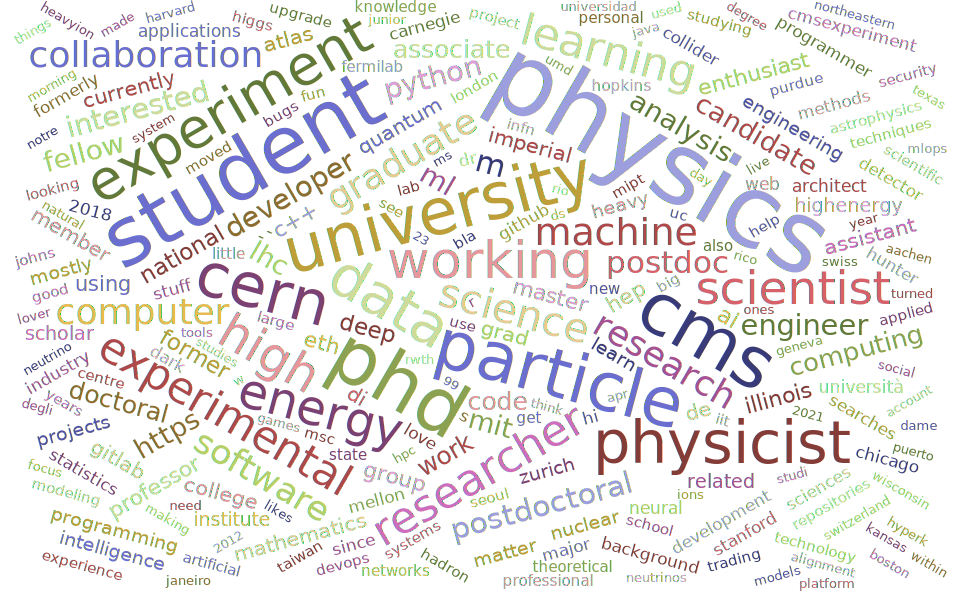
\includegraphics[width=\linewidth]{PLOTS/cmssw-profile-bios-wordcloud.pdf}

\begin{center}
\begin{minipage}{0.9\linewidth}
A lot of ``physics,'' ``student,'' ``particle,'' ``physicist,'' ``PhD,'' ``CERN,'' and ``CMS.''
\end{minipage}
\end{center}

\column{0.55\linewidth}
\mbox{ } \hfill \textcolor{darkblue}{\large Selected by ROOT interaction} \hfill \mbox{ }

\vspace{0.2 cm}
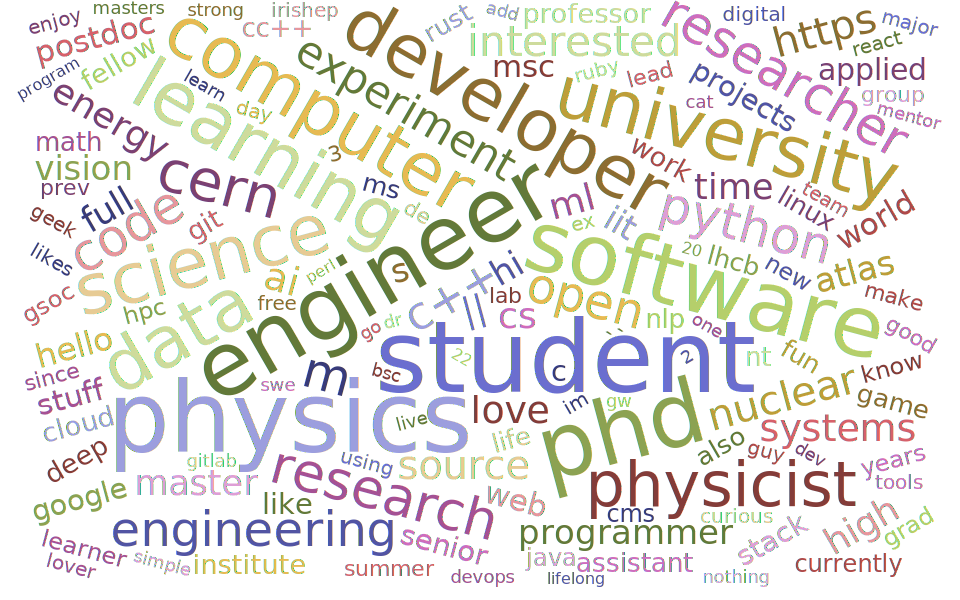
\includegraphics[width=\linewidth]{PLOTS/root-repo-profile-bios-wordcloud.pdf}

\begin{center}
\begin{minipage}{0.95\linewidth}
A little more ``software,'' ``engineer,'' but still lots of ``physics,'' ``student,'' and ``PhD.''
\end{minipage}
\end{center}

\end{columns}
\end{frame}


\end{document}
